\documentclass{report}
\usepackage[margin=1in, paperwidth=8.5in, paperheight=11in]{geometry}
%Math packages%
\usepackage{amsmath}
\usepackage{amsthm}
%Spacing%
\usepackage{setspace}
\onehalfspacing
%Lecture number%
\newcommand{\lectureNum}{9}
%Variables - Date and Course%
\newcommand{\curDate}{January 31, 2017}
\newcommand{\course}{CS 251}
\newcommand{\instructor}{Stephen Mann}
%Defining the example tag%
%\theoremstyle{definition}%
\newtheorem{ex}{Example}[section]
%Setting counter given the lecture number%
\setcounter{chapter}{\lectureNum{}}
%Package to insert code%
\usepackage{listings}
\usepackage{courier}
\usepackage{xcolor}
\lstset { %
    tabsize=2,
    breaklines=true,
    language=C++,
    backgroundcolor=\color{blue!8}, % set backgroundcolor
    basicstyle=\footnotesize\ttfamily,% basic font setting
}
%Package used to draw circuits%
\usepackage{circuitikz}
\begin{document}
%Note title%
\begin{center}
\begin{Large}
\textsc{\course{} | Lecture \lectureNum{}}
\end{Large}
\end{center} 
\noindent \textit{Bartosz Antczak} \hfill
\textit{Instructor: \instructor{}} \hfill
\textit{\curDate{}}
\rule{\textwidth}{0.4pt}
% Actual Notes%
\section{Operations on Numbers in Floating-Point Representation}
\subsubsection{Floating-Point Addition}
Consider $9.54 \times 10^2 + 6.83 \times 10^1$ (assume we can only round to two digits). To add these two numbers:
\begin{enumerate}
\item Match the exponents ($9.54 \times 10^2 + .683 \times 10^2$)
\item Add significands, with sign: $10.223 \times 10^2$
\item Normalize: $1.0223 \times 10^3$
\item Check for exponent overflow/underflow
\item Round: $1.02 \times 10^3$
\end{enumerate}
\subsubsection{Floating-Point Multiplication}
Consider $(9.54 \times 10^2) \times (6.83 \times 10^1)$ (assume we can only round to two digits). To add these two numbers:
\begin{enumerate}
\item Add exponents: $2 + 1 = 3$
\item Multiply significands: $9.54 \times 6.83 = 65.1582$
\item Normalize: $6.51582 \times 10^4$
\item Check for exponent overflow/underflow
\item Round: $6.52 \times 10^4$
\item Set sign
\end{enumerate}
\subsection{Accuracy of Floating-Point Numbers}
The biggest problem with accuracy is a round-off error (e.g., using a calculator to disprove Fermat's last theorem). The result of an operation cannot be represented precisely, which means that the result must be rounded. \textbf{In this class, we'll round 1/2 up}.\\
For $n-$bit accuracy, we need to keep $n+2$ bits during the computation.\newpage
\section{Single-Cycle Processor Implementation}
We will implement small subsets of MIPS operations, such as \texttt{lw}, \texttt{sw}, and \texttt{add}.
\subsubsection{Instruction Format}
%TODO include pic from 4.5%
\begin{figure}[ht]
\begin{center}
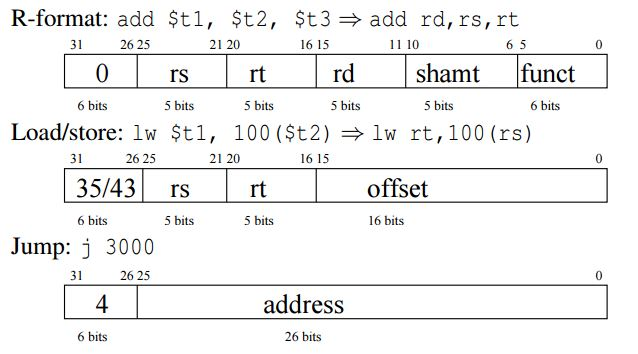
\includegraphics[scale=0.5]{bitlayout.jpg}
\end{center}
\caption{The 32-bit layout for each respective MIPS instruction. Courtesy of Prof. Mann's slides.}
\end{figure}
%END%
\end{document}